% Nama kelompok : 3
% Kelas : D4 Teknik Informatika 3C
% 1. Kezia Tirza Naramessakh (1154093)
% 2. Mariani Rospilinda Siki (1154107)
% 3. Doli Jonviter Nt Simbolon (1154016)
% 4. Benedictus Simantupang (1154116)
% 5. Dimas Mathovani 


\section{Koordinat Lintang Utara, Lintang Selatan, Bujur Timur, Bujur Barat}
Koordinat digunakan untuk menunjukkan suatu titik di Bumi berdasarkan garis lintang dan garis bujur. Koordinat dibagi menjadi dua bagian irisan yaitu irisan melintang yang disebut dengan garis lintang mulai dari khatulistiwa, membesar ke arah kutub(utara maupun selatan) sedangkan yang lain membuju r mulai dari garis Greenwhich membesar ke arah barat dan timur. Satuan skala koordinat dibagi dalam derajat lintang 0* sampai 90* dan bujur 0* sampai 180*. Koordinat ini ditulis dalam satuan derajat, menit, dan detik, misalnya 110*35'32", dan seterusnya. Untuk membagi dunia dalam wilayah utara dan selatan, maka ditentukan sebuah garis yang tepat berada di tengah, yaitu garis Equator / Khatulistiwa. Untuk membagi wilayah timur dan barat, maka ditentukan sebuah garis Prime meridian yang terletak di kota Greenwich (Inggris), dan perpotongannya bertemu di wilayah laut pasific, yakni memotong kepulauan Fiji.
Koordinat pada gambar \ref{Koordinat} di jelaskan garis Lintang dan Bujur
\begin{figure}[ht]
	\centerline{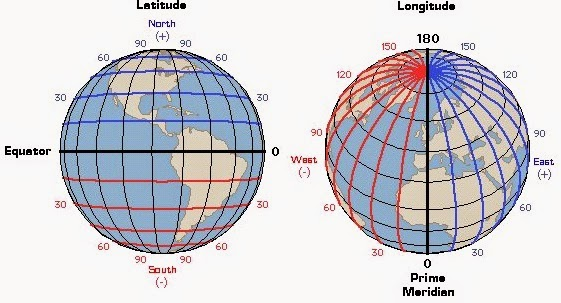
\includegraphics[width=1\textwidth]{figures/Koordinat.JPG}}
	\caption{Koordinat Lintang dan Bujur}
	\label{Koordinat}
	\end{figure}

\subsection{Sistem Koordinat}
Dalam artikel Zuhdi menjelaskan Koordinat dimaksudkan untuk memberikan pengalamatan terhadap setiap lokasi di permukaan bumi. Pengalamatan dengan sistem koordinat didasarkan atas jarak timur-barat dan utara-selatan suatu tempat dari suatu titik pangkal tertentu. Jarak diukur dalam satuan derajat sudut yang dibentuk dari titik pangkal ke posisi tersebut melalui pusat bumi. Sedangkan titik pangkal ditetapkan berada di perpotongan belahan utara-selatan bumi (garis khatulistiwa) dengan garis yang membelah bumi timur-barat melalui kota GreenWhich di Inggris. 
Untuk lebih jelas tentang bentuk titik koordinat lihat pada gambar \ref{sistemkoordinat} dibawah ini :
\begin{figure}[ht]
	\centerline{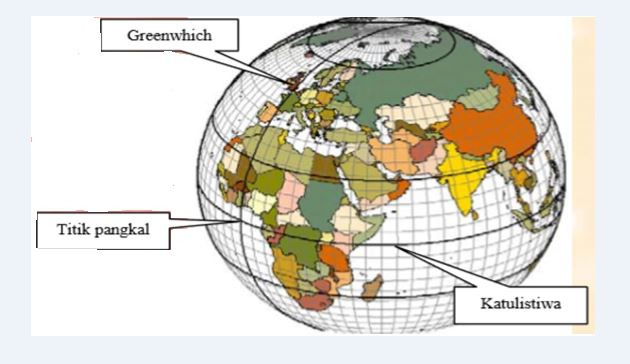
\includegraphics[width=1\textwidth]{figures/sistemkoordinat.JPG}}
	\caption{Bentuk titik Koordinat}
	\label{sistemkoordinat}
	\end{figure}

Baik garis lintang maupun garis bujur diukur dalam derjat dan dibagi lagi dalam menit dan detik. 1 derajat garis bujur diukur lapangan sama dengan 11,32 km. Satuan derajat bisa juga disebut jam sehingga setiap derajat terbagi menjaid 60 menit dan setiap menit terbagi menjadi 60 detik. Dalam penulisan letak astronomis contohnya 60 derajat 23' 15"S, maka dibaca sebagai 60 derajat 23 menit 15 detik lintang selatan. pada sistem pemetaan internasional huruf U sebagai lintang utara diganti dengan huruf N (north). Besar sudut dalam sistem koordinat geografik dapat dinyatakan dalam dua cara, yaitu dengan satuan DMS(Degree Minute Second) atau satuan DD(Decimal Degree), dalam sistem satuan DMS, setiap derajat sudut dibagi menjadi 60 menit dan setiap menitnya dibagi lagi menjadi 60 detik. Penulisannya dinyatakan sebagai dd°mm'ss". Sedangkan pada sistem satuan setiap derajatnya dinyatakan dalam pecahan decimal (pecahan berkoma). Baik dalam DMS maupun DD, perlu diketahui berapa ketelitian suatu nilai koordinat. Karena di wilayah khatulistiwa jarak 1° sama dengan jarak 111321 meter. Maka perlu diperhatikan keselahan yang terjaddi jika kita mengabaikan suatu angka menit atau detik pada DMS atau suatu nilai digit dalam koordinat DD. Pada sistem DD, perlu diperhatikan jarak yang diwakili oleh setiap digit dibelakang koma. Perubahan satu satuan padaa digitt pertamma dii belakang koma mempunyai nilai jarak lebih dari 11 Km. Perubahan satu unit pada digit keduat dibelakang koma berarti 1,1 Km. Demikian seterusnya. Berarti jika kita misalnya hanya mentolerir kesalahan sampai 100 m, maka koordinat DD harus dibuat setidaknya sampai 4 digit di belakang koma. Kombinasi antara garis lintang dan garis bujur akan membentuk sutau koordinat lokasi di permukaan bumi dengan sumbu x sebagai garis lintang dan sumbu y sebagai garis bujur dalam koordinat kartesius. Pada Bujur/Longitude (X) merupakan garis yang perpindahannya secara vertical dan pada Lintang/Lattitude (Y) merupakan garis yang mempunyai perpindahan secara horizontal. \cite{zuhdi2012sistem}.

Lihat pada gambar \ref{lintangbujur} dibawah ini :
\begin{figure}[ht]
	\centerline{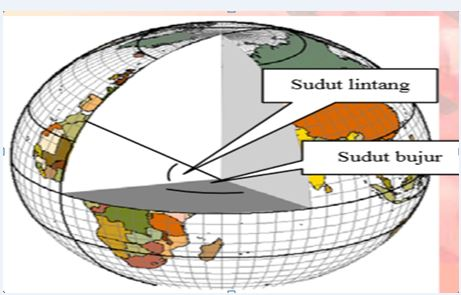
\includegraphics[width=1\textwidth]{figures/lintangbujur.JPG}}
	\caption{Titik Lintang dan Bujur}
	\label{lintangbujur}
	\end{figure}

\subsubsection{Garis Lintang}
Sebuah garis khayal yang digunakan untuk menentukan lokasi di Bumi terhadap garis khatulistiwa(utara atau selatan). Posisi lintang merupakan penghitungan sudut dari 0 derajat di khatulistiwa sampai ke +90 derajat di kutub utara dan -90 derajat di kutub selatan. Dalam bahasa indonesia lintang di sebelah utara khatulistiwa diberi nama Lintang Utara(LU), demikian pula lintang di sebelah selatan khatulistiwa diberi nama Lintang Selatan(LS). Lintang Utara dan Lintang Selatan menyatakan besarnya sudut antara posisi lintang dengan garis Khatulistiwa. Garis Khatulistiwa sendiri adalah lintang 0 derajat. 
Nilai koordinat lingtang dimulai dari garis lingkaran khatulistiwa yang diberi nilai 0 derajat. Selanjutnya garis lintang yang lain berupa lingkarang paralel (sejajar) katulistiwa berada disebelah utara dan selatan khatulistiwa. Lingkaran paralel di selatan disebut garis lintang selatan (LS) dan diberi nilai negatif, sedangkan lingkaran paralel diutara diberi nilai positif dan disebut garis lintang utara (LU). Nilai maksimum koordinat garis lintang adalah 90 derajat yaitu terletak di kutub-kutub bumi. 
Lingkaran paralel merupakan representasi garis lintang ini semakin mengecil ukurannya dengan semakin jauh dari katulistiwa. sehingga jarak 1 derajat timur-barat dari katulistiwa jauh lebih besar dari pada jarak 1 derajat timur-barat di tempat yang jauh dari katulistiwa. Di khtulistiwa 1 derajat timur-barat sama dengan 111.321 km, tapi di dekat kutub 1 derajat timur-barat hanya beberapa meter saja. itu sebabnya grid yang dibuat dari garis lintang dan garis bujur, tampak berupa sangkar dikatulistiwa dan berubah menjadi persegi didaerah kutub
lintang memiliki symbol phi dan menunjukkan sudut antara garis lurus dititik tertentu dengan bidang ekuator. Lintang ditentukan dalam angka derajat dimulai dari 0 derajat dan berakhir dengan 90 derajat. garis lintang ini membagi bumi menjadi belahan bumi utara dan selatan. garis ekuator atau khatulistiwa berada di lintang 0 derajat. Garis lintang biasa digunakan untuk melihat penyebaran iklim di bumi.
Latitude aau garis lintang adalah garis yang menentukan lokasi berada di sebelah utara atau selatan ekuator. garis lintang diukur mulai dari titik 0 derajat dari khatulistiwa sampai 90 derajat di kutub. Garis lintang digunakan untuk membatasi corak iklim di permukaan bumi, berikut ini merupakan pembagian iklim di bumi menurut batas garis lintang:
1. 23,5-23,5 LU/LS = iklim tropis
2. 23,5-40 LU/LS = iklim subtropis
3. 40 Lu-66,5 LU/LS = iklim sedang
4. 66,5-90 LU/LS = iklim kutub
Indonesia terletak antara 6 derajat Lintang Utara (LU) – 11 derajat Lintang Selatan (LS) dan diantara 95 derajat bujur timur – 141 derajat Bujur timur.
Adapun wilayah indonesia itu pada bagian paling utara yang ebrada di Pulau Weh di Nanggroe Aceh Darussalam yang terletak pada 6 derajat lintang utara, dan untuk daerah indonesia yang paling berada di selatan yaitu Pulau Roti di Nusa Tenggara Timur yang terletak pada 11 derajat lintang selatan. Kemudian mengacu pada letak lintangnya, di wilayah Indonesia berada pada 6 derajat lintang utara – 11 derajat lintang selatan, hal tersebut disebabkan indonesia mempunyai iklim tropis dengan beberapa ciri-ciri yaitu mempunyai hutan hujan tropis yang begitu luas dan mempunyai nilai ekonomis yang sangat tinggi, mendapatkan sinar matahari yang lama setiap sepanjang tahun, mempunyai curah hujan yang tinggi dan memiliki banyak penguapan sehingga akan meningkatkan kelembaban udara.
Pada gambar \ref{lintang} dijelaskan titik koordinat Lintang pada sumbuh Y :
\begin{figure}[ht]
	\centerline{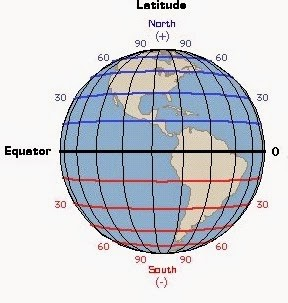
\includegraphics[width=1\textwidth]{figures/lintang.JPG}}
	\caption{Titik koordinat Lintang pada sumbuh Y}
	\label{lintang}
	\end{figure}

\subsubsection{Garis Bujur}
Menggambarkan lokasi sebuah tempat di timur atau barat Bumi dari sebuah garis utara-selatan yang disebut Meridian Utama. Longitude diberikan berdasarkan pengukuran sudut yang berkisar dari 0 derajat Meridian Utama ke +180 derajat arah timur dan -180 derajat arah barat. Tidak seperti lintang yang memiliki ekuator sebagai posisi awal alami, tidak ada posisi awal alami untuk bujur. Bujur di sebelah barat Meridian diberi nama Bujur Barat(BB), demikian pula bujur di sebelah timur Meridian diberi nama Bujur Timur(BT).
Nilai koordinat garis bujur dimulai dari bujur 0 derajat yaitu Greenwhich, kemudian memebersasr ke arah timur dan barat sampai bertemu kembali di garis batas tanggal internasional yaitu terletak di selat bering dnegan nilai 180 derajat. garis bujur 0 derajat disebut prime meridian atau meridian greenwhich. garsi bujur ke arah barat diberi nilai negatif dan disebut bujur barat (west longitude) serta disingkan BB. sedangkan garis bujur yang ke arah timur diberi nilai positif dan disebut bujur timur (east longitude) disingkat BT. nilai koordinatnya didasarkan atas besarnya sudut yang terbentuk dari bujur 0 ke garis bujur tersebut melalui pusat bumi.
Longitude atau garis bujur memiliki symbol lamda. garis bujur ini merupakan garis yang menunjukkan bagian barat dan timur dilihat dari titik pangkal yaitu di greenwich meridian. garis bujur emiliki batas maksimum yaiu 180 derajat ke arah timur dar GMT dan 180 derajat ke arah barat dari GMT. keduanya bertemu di garis internasional date line disekitar pasifik.
longitude atau garis bujur digunakan untuk menentukan lokasi diwilayah barat atau timur dari garis utara selatan yang sering disebut juga garis meridian. garis bujur digunakan untuk menentukan waktu dan tanggal.
Titik di barat bujur 0° dinamakan Bujur Barat sedangkan titik di timur 0° dinamakan Bujur Timur. Kombinasi garis lintang dan garis bujur ini berguna untuk menentukan suatu lokasi di permukaan bumi. Garis Lintang menandakan sumbu y dan garus bujur menandakan sumbu x dalam sistem koordinat cartesian. Sebagi contoh kota Sabang di pulau We berada pada koordinat 6oLU 95o BT, dan kota Merauke di Papua memiliki koordinat 11oLS dan 141oBT.
Indonesia berada pada 95 derajat bujur timur – 141 derajat bujur timur menyebabkan Indonesia mempunyai tiga waktu dan pada setiap waktu memiliki daerah tersendiri, sehingga Indonesia memiliki beberapa pembagian waktu yaitu Waktu Indonesia bagian timur atau WIT mencakup Papua, kepulauan Maluku dan pulau-pulau kecil disekitarnya. Untuk waktu indonesia bagian  timur mempunyai selisih waktu sebanyak 9 jam lebih awal dari Greenwich Mean time atau GMT. Kemudian untuk Waktu Indonesia bagian tengah atau WITA mencakup Nusa tenggara, kalimantan selatan, Pulau Sulawesi, Bali dan pulau-pulau kecil yang ada disekitarnya. Untuk Indonesia bagian tengah mempunyai selisih waktu sebanyak 8 jam yang lebih awal dari Greenwich mean time (GMT). Kemudian, untuk daerah waktu Indonesia bagian barat atau WIB yang mencakup Madura, Jawa, kalimantan barat, kalimantan tengah, Sumatera dan pulau-pulau kecil yang ada disekitarnya. Adapun waktu indonesia bagian barat mempunyai selisih waktu sebanyak 7 jam yang lebih awal dari Greenwich mean time.
Pada gambar \ref{bujur} dijelaskan titik koordinat Lintang pada sumbuh X :
\begin{figure}[ht]
	\centerline{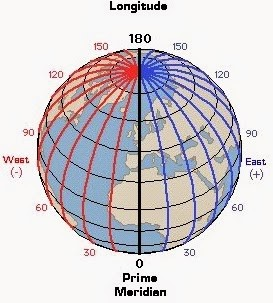
\includegraphics[width=1\textwidth]{figures/bujur.JPG}}
	\caption{Titik koordinat Bujur pada sumbuh X}
	\label{bujur}
	\end{figure}